\documentclass[notes]{subfiles}
\begin{document}
	\addcontentsline{toc}{section}{1.3 - Functions with Unbounded Input}
	\refstepcounter{section}
	\fancyhead[RO,LE]{\bfseries \large \nameref{cs13}} 
	\fancyhead[LO,RE]{\bfseries \currentname}
	\fancyfoot[C]{{}}
	\fancyfoot[RO,LE]{\large \thepage}	%Footer on Right \thepage is pagenumber
	\fancyfoot[LO,RE]{\large Chapter 1.3}


\section*{Functions with Unbounded Input}\label{cs13}
	\subsection*{Motivating Example}
		Consider the function $f(x) = \dfrac{1}{x-2}$, graphed below:
		\begin{center}
			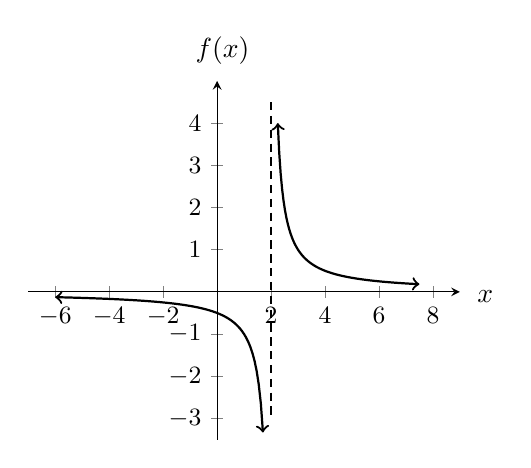
\begin{tikzpicture}
				\begin{axis}[
					scale = .8,
					every tick label/.append style={font=\small},
					axis x line = middle,
					axis y line = middle,
		    			every axis y label/.style={at={(ticklabel cs:1.15)}},
		    			ytick = {-3, -2, -1, 1, 2, 3, 4},
						y label style={at={(axis description cs:.45,1.15)},anchor=north},
		    			ylabel = {$f(x)$},
		    			ymin = -3.5, ymax = 5,
	    				every axis x label/.style= {at ={(ticklabel cs:1)}},
	    				xtick = {-6, -4, -2,2,4,6,8},
	    				x label style={at={(axis description cs:1.1,.4)},anchor=east},
	    				xlabel = {$x$},
	    				xmin = -7, xmax = 9			
				]
					\addplot[<->,thick, samples = 100, domain = -6.:1.7] {1/(x-2)};
					\addplot[<->,thick, samples = 100, domain = 2.25:7.5] {1/(x-2)};
					\coordinate (bottom) at (2,-3);
					\coordinate (top)at (2,4.5);
				\end{axis}
				\draw[densely dashed] (top)--(bottom);
			\end{tikzpicture}
		\end{center}
		\begin{enumerate}[(a)]
			\item What happens to the output of $f$ as the input increases without bound?  Write your answer in limit notation.
				\vs{.75}
			\item What happens to the output of $f$ as the input decreases without bound?  Write your answer in limit notation.
				\vs{.75}
			\item What happens to the output of $f$ at $x =2$?
				\vs{.75}
		\end{enumerate}

	\subsection*{Left/Right Hand Limits}
		\begin{defn}[Left/Right Hand Limit]
			Let $f$ be a function defined on an interval containing some constant $c$ (except possibly at $c$ itself).\\
				\tabitem If $f(x)$ approaches the value of $L_1$ as $x$ approaches $c$ from the left, then the \textbf{left-hand limit} of $f$ is $L_1$, and is written \showto{ins}{\fbox{$\ds \lim_{x\to c^-} f(x) = L_1$}\\ }\showto{st}{\vspace*{.6in}}
		
				\tabitem If $f(x)$ approaches the value of $L_2$ as $x$ approaches $c$ from the right, then the \textbf{right-hand limit} of $f$ is $L_2$, and is written \showto{ins}{\fbox{$\ds \lim_{x\to c^+} f(x) = L_2$}}\showto{st}{\vspace*{.4in}}
		\end{defn}
		
		\begin{ex}
			For $f(x) = \dfrac{1}{x-2}$, find $\ds \lim_{x\to 2^-} f(x)$ and $\ds \lim_{x\to 2^+} f(x)$.
		\end{ex}
			\vs{1}
		\begin{ex}
			$ $\\ Use a calculator to numerically examine the limit behavior of $f(x) = \dfrac{1}{x-2}$ at $x = 2$.  \\
			\begin{flushleft}
				\begin{minipage}{.4\textwidth}
				%\tabulinesep=.25mm
				\begin{tabu}{|X[0.5,c]|X[1,c]|}\hline
						$x$ & $f(x)$ \\ \hline
							& \\
					1.9		& \\
							& \\ \hline
							& \\
					1.99	& \\
							& \\ \hline
							& \\
					1.999	& \\
							& \\ \hline
							& \\
					1.9999	& \\
							& \\ \hline
							& \\
					1.99999	& \\
							& \\ \hline\hline
							& \\
					$\ds \lim_{x\to 2^-}f(x) = $ & \\
												& \\ \hline			
				\end{tabu}
				\end{minipage}
				\begin{minipage}{.4\textwidth}
				%\tabulinesep=.5mm
				\begin{tabu}{|X[.5,c]|X[1,c]|}\hline
						$x$ & $f(x)$ \\ \hline
							& \\
					2.1		& \\
							& \\ \hline
							& \\
					2.01	& \\
							& \\ \hline
							& \\
					2.001	& \\
							& \\ \hline
							& \\
					2.0001	& \\
							& \\ \hline
							& \\
					2.00001	& \\
							& \\ \hline\hline
							& \\
					$\ds \lim_{x\to 2^+}f(x) = $ & \\
												& \\ \hline				
				\end{tabu}
				\end{minipage}
				\begin{minipage}{.15\textwidth}
					$\ds \lim_{x\to 2} f(x) =$\\[35pt]\makebox[1.2in]{\hrulefill}
				\end{minipage}
			\end{flushleft}
		\end{ex}		
			\newpage
			
		\begin{ex} \label{discontinuity} Use the graph of $g$ to answer the following: 
			\begin{center}
			\begin{minipage}{.45\textwidth}
				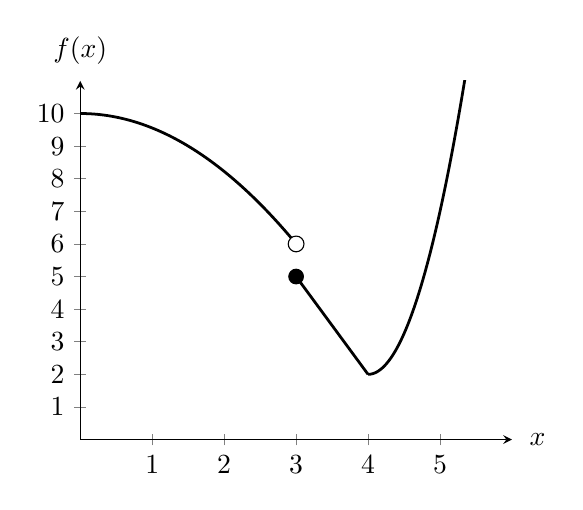
\begin{tikzpicture}
				\begin{axis}[
					scale = .8,
					axis x line = middle,
					axis y line = middle,
	    			every axis y label/.style={at={(ticklabel cs:1.15)}},
	    			ytick = {1,2,...,10},
					y label style={at={(axis description cs:0,1.15)},anchor=north},
	    			ylabel = {$f(x)$},
	    			ymin = 0, ymax = 11,
    				every axis x label/.style= {at ={(ticklabel cs:1)}},
    				xtick = {1,2,3,4,5},
    				x label style={at={(axis description cs:1.1,0)},anchor=east},
    				xlabel = {$x$},
    				xmin = 0, xmax = 6			
				]
					\addplot [line width=1pt,smooth,samples=100,domain=0.:2.93] {(-.444)*x^2 + 10}; % plots first piece of function
					\coordinate (circle1) at (3,6);
					\addplot[line width = 1pt, smooth, samples = 100, domain = 3.0:4.0] {-3.*x + 14.}; %plot second piece
					\coordinate (circle2) at (3,5);
					\addplot[->,line width = 1pt, smooth, samples = 100, domain = 4.0:6.0] {5*(x - 4)^2 + 2}; %plot third piece
				\end{axis}
				\fill[white] (circle1) circle (.1);
				\draw (circle1) circle (.1);
				\fill (circle2) circle (.1);
			\end{tikzpicture}
			\end{minipage}\hspace{20pt}
			\begin{minipage}{.45\textwidth}
				\begin{multicols}{2}
				\setlength\columnsep{50pt}
				\begin{enumerate}[(a)]
					\item $\ds \lim_{x\to 4^-} g(x)=$\\ \\ \\
					\item $\ds \lim_{x\to 4^+} g(x)=$\\ \\ \\
					\item $\ds \lim_{x\to 4} g(x)=$\\ \\
					\item $\ds \lim_{x\to 3^-} g(x)=$\\ \\ \\
					\item $\ds \lim_{x\to 3^+} g(x)=$\\ \\ \\
					\item $\ds \lim_{x\to 3} g(x)=$\\ \\
				\end{enumerate}
				\end{multicols}
			\end{minipage}
			\end{center}
		\end{ex}
			%\vs{.5}

		\begin{ex}
			Examine the limit behavior of the function $g(t) = \dfrac{3t^2-9}{t-3}$ at $t = 3$.  Round to the nearest tenth if necessary.
		\end{ex}
			\vs{1}
			
			\newpage
			
		\begin{ex}
			Use a calculator to examine the limit behavior of the function $r(p) = \dfrac{p^2-64}{p+8}$ at $p = -8$.  Round to the nearest thousandth if necessary.
		\end{ex}
			\vs{1}
			

		\begin{ex}
			Use a calculator to examine the limit behavior of the function $P(y) = \dfrac{3^y}{2y-5}$ at $y = 2.5$.  Round your answer to 2 decimal places.
		\end{ex}
			\vs{1}
			\newpage
				
	\subsection*{Continuity}
		\begin{defn}[Continuity]
			A function $f(x)$, defined on some input interval containing $c$, is said to be \textbf{continuous} at $c$ if and only if the following conditions are satisfied:\\
			\begin{enumerate}[(1)]
				\item \showto{ins}{\fbox{$\ds \lim_{x\to c} f(x)$ exists}}\showto{st}{$ $\vspace*{.4in}}
				\item \showto{ins}{\fbox{$f(c)$ exists}}\showto{st}{$ $\vspace*{.4in}}
				\item \showto{ins}{\fbox{$\ds \lim_{x\to c} f(x) = f(c)$}}\showto{st}{$ $\vspace*{.4in}}
			\end{enumerate}
			A function is continuous on any open interval $(a,b)$ if it is continuous at every point inside the interval.  If a function is not continuous at the input $x = c$, then we say that $f$ is \showto{ins}{\fbox{discontinuous}}\showto{st}{\\[25pt] \\ \blank{2}} at $c$.
		\end{defn}

		\begin{ex}
			Identify any points of discontinuity in the function $f(x) = \dfrac{1}{x-2}$.  Explain why the function is discontinuous at those points.
		\end{ex}
			\vs{1}
		\begin{ex}
			Identify any points of discontinuity in the function $g(x)$ in Example 3.\ref{discontinuity}.  Explain why the function is discontinuous at those points.
		\end{ex}
			\vs{1}			
			\newpage

		\begin{ex}
		Use the graph to find the following:
		\begin{center}
			\begin{tikzpicture}
				\begin{axis}[
					scale = 1.5,
					every tick label/.append style={font=\small},
					axis x line = middle,
					axis y line = middle,
		    			every axis y label/.style={at={(ticklabel cs:1.15)}},
		    			ytick = {-4, -2, -3, -1, 1, 2, 3, 4},
					y label style={at={(axis description cs:.5,1.15)},anchor=north},
		    			ylabel = {$f(x)$},
		    			ymin = -5, ymax = 5,
	    				every axis x label/.style= {at ={(ticklabel cs:1)}},
	    				xtick = {-4,-3,-2,-1,1,2,3,4},
	    				x label style={at={(axis description cs:1.1,.5)},anchor=east},
	    				xlabel = {$x$},
	    				xmin = -5, xmax = 5			
					]
					\addplot[<-,thick,smooth,domain = 1.4:3.] {4/(x-1)-5};
					\addplot[->,thick,smooth,domain = 3.:4.9] {x-6};
					\addplot[<-,thick,smooth, domain = -4.9:1]  {2^x -4};
					\coordinate (circle1) at (1,-2);
					\coordinate (circle2) at (3,-3);
					\coordinate (circle3) at (3,2);
				\end{axis}
					\fill[white] (circle1) circle (.1);
					\draw[thick] (circle1) circle (.1);
					\fill[white] (circle2) circle (.1);
					\draw[thick] (circle2) circle (.1);
					\fill (circle3) circle (.1);
			\end{tikzpicture}
		\end{center}\vspace*{20pt}
		\begin{minipage}{\textwidth}
			\begin{multicols*}{3}
			\begin{enumerate}[(a)]
				\item $\ds \lim_{x\to 1^+} f(x)$\\[50pt]
				\item $\ds \lim_{x\to 1^-} f(x)$\\[50pt] 
				\item $\ds \lim_{x\to 1} f(x)$\\[50pt] 
				\item Is $f$ continuous at $x =1 $?\\[50pt]
					\columnbreak
				\item $\ds \lim_{x\to 3^+} f(x)$\\[50pt] 
				\item $\ds \lim_{x\to 3^-} f(x)$\\[50pt]  
				\item $\ds \lim_{x\to 3} f(x)$\\[50pt] 
				\item Is $f$ continuous at $x =3 $?\\[50pt]
					\columnbreak
				\item $\ds \lim_{x\to 0^+} f(x)$\\[50pt] 
				\item $\ds \lim_{x\to 0^-} f(x)$\\[50pt]  
				\item $\ds \lim_{x\to 0} f(x)$\\[50pt] 
				\item Is $f$ continuous at $x =0 $?\\[50pt]
			\end{enumerate}
				\raggedcolumns
			\end{multicols*}
		\end{minipage}
		\end{ex}
			\newpage

	\subsection*{Properties of Limits}
		Let $f(x)$ and $g(x)$ be continuous functions over some input interval containing $c$, and $k$ be some arbitrary constant.  Then, we have the following properties of limits:
		\begin{enumerate}[(1)]
			\item Constant Rule: \showto{ins}{\fbox{$\ds \lim_{x\to c} k = k$}}\showto{st}{$ $\vspace*{.9in}}
			\item Sum Rule: \showto{ins}{\fbox{$\ds \lim_{x\to c}\left[f(x) + g(x)\right] $}}\showto{st}{$ $\vspace*{.9in}}
			\item Constant Multiple Rule: \showto{ins}{\fbox{$\ds \lim_{x\to c} \left[k\cdot f(x)\right] = k\lim_{x\to c} f(x) $}}\showto{st}{$ $\vspace*{.9in}}
			\item Replacement Rule: If $f(c)$ is defined at $c$, then \showto{ins}{\fbox{$\ds \lim_{x\to c}f(x) = f(c)$}}\showto{st}{$ $\vspace*{.9in}}
			\item Product Rule: \showto{ins}{\fbox{$\ds\lim_{x\to c} \left[f(x)\cdot g(x)\right] = \left[\lim_{x\to c} f(x)\right]\cdot\left[\lim_{x\to c}g(x)\right]$}}\showto{st}{$ $\vspace*{.9in}}
			\item Quotient Rule: \showto{ins}{\fbox{$\ds \lim_{x\to c} \left[\dfrac{f(x)}{g(x)}\right] = \dfrac{\ds\lim_{x\to c} f(x)}{\ds\lim_{x\to c} g(x)}$ (as long as $\ds\lim_{x\to c} g(x)\neq 0$)}}\showto{st}{$ $\vspace*{.9in}}
			\item If $f(x)$ can be factored as $f(x) = h(x)\cdot k(x)$, and $g(x)$ can also be factored as $g(x) = j(x)\cdot k(x)$, then
				\[\lim_{x\to c} \frac{f(x)}{g(x)} = \lim_{x\to c}\frac{h(x)\cdot k(x)}{j(x) \cdot k(x)} = \lim_{x\to c} \frac{h(x)}{j(x)}\]
				i.e. common factors may be canceled across fractions under the limit
		\end{enumerate}
			\newpage

		\begin{ex}
			Algebraically determine the limits of the following:
			\begin{enumerate}[(a)]
				\item $\ds\lim_{x\to 5} 9$
					\vs{1}
				\item $\ds\lim_{z\to 3} (4z-5)$
					\vs{1}
				\item $\ds\lim_{t\to -3} \dfrac{t^2-4t-21}{t+3}$
					\vs{1}
				\item $\ds\lim_{m\to 13} \dfrac{m}{m^2+4m}$
					\vs{1}
				\item $\ds\lim_{h\to 0} \dfrac{(3+h)^2 -9}{h}$
					\vs{1}
			\end{enumerate}
		\end{ex}
		
		\begin{ex}
			Determine the limit: $\ds \lim_{h\to 0} \dfrac{(5+h)^2-25}{h}$
		\end{ex}
			\vs{1}
			\newpage

		\begin{ex}
			Let $f(x) = \begin{cases} x^2 & x < -1 \\ 1 & x\geq -1\end{cases}$.  \textbf{Algebraically} determine the following limits and answer the questions:
			\begin{enumerate}[(a)]
				\item $\ds \lim_{x\to -1^-} f(x)$
					\vs{1}
				\item $\ds \lim_{x\to -1^+} f(x)$
					\vs{1}
				\item $f(-1)$
					\vs{1}
				\item Is $f$ continuous at $x = -1$?  Why?
					\vs{1}
				\item Graph $f(x)$. Do your answers make sense?
					\vs{1}
			\end{enumerate}
		\end{ex}
			\newpage

		\begin{ex}
			Let $h(t) = \begin{cases} 3^t - 9 & t < 2 \\ t^2-4 & t\geq 2\end{cases}$.  \textbf{Algebraically} determine the following limits and answer the questions:
			\begin{enumerate}[(a)]
				\item $\ds \lim_{t\to 2^-} h(t)$
					\vs{1}
				\item $\ds \lim_{t\to 2^+} h(t)$
					\vs{1}
				\item $h(2)$
					\vs{1}
				\item Is $h$ continuous at $t = 2$?  Why?
					\vs{1}
				\item Graph $h(t)$. Do your answers make sense?
					\vs{1}
			\end{enumerate}
		\end{ex}
	\clearpage
\end{document}